\documentclass[10pt]{article}
\usepackage{polski}
\usepackage[utf8]{inputenc}
\usepackage{graphicx}
\title{Sprawozdanie z projektu związanego z algorytmami operującymi na grafach}
\author{Adrian Nowosielski\\Cezary Skorupski}
\date{02.06.2022}
\begin{document}
\maketitle
\thispagestyle{empty}
\newpage
\thispagestyle{empty}
\begin{center}
    \textbf{\Large{Streszczenie}}\\
    Dokument stanowi sprawozdanie z projektu \textbf{Grafy} realizowanego w ramach zajęć projektowych na Politechnice Warszawskiej. Sprawozdanie zawiera wyszczególniony opis aktualnego stanu projektu, zmiany w programie względem specyfikacji funkcjonalnej oraz wnioski z pracy nad projektem w języku Java.
\end{center}
\newpage
\newpage
\begin{center}
    \tableofcontents
    \thispagestyle{empty}
\end{center}
\newpage
\pagenumbering{arabic}
\section{Zarys projektu}
Projekt \textbf{Grafy} w języku Java zakłada stworzenie programu, który będzie generował grafy w postaci kratki. Skrzyżowania kratek to węzły, a linie pionowe i poziome to krawędzie. Dodatkowo badane grafy są ważone, czyli takie, w których każdej krawędzi przypisana jest pewna wartość liczbowa dodatnia. W ramach projektu zespół miał na celu zaimplementowanie:
\begin{itemize}
    \item Generowanie opisanego grafu w kratkę do pliku .txt z opisanym w specyfikacji funkcjonalnej formacie zapisu grafu.
    \item Czytanie grafu w kratkę z pliku o określonym w specyfikacji funkcjonalnej formacie.
    \item Algorytmu Breadth First Search-algorytmu umożliwiającego sprawdzenie, czy podany przez użytkownika graf jest spójny.
    \item Algorytmu Dijkstra-algorytmu umożliwiającego znalezienie najkrótszej drogi pomiędzy wybranymi przez użytkownika wierzchołkami.
    \item Stworzenia graficznego interfejsu użytkownika, na którm użytkownik ma możliwość wygenerowania grafu w kratkę na ekranie.
    \item Możliwość wyboru węzłów do wyznaczania najkrótszej ścieżki za pomocą myszki.
    \item Narysowanie najkrótszej ścieżki pomiędzy węzłami, wybranymi przez użytkownika.
\end{itemize}
Krokiem, z którym zespół musi się na końcu zmierzyć, to napisanie  dokumentu sprawozdania podsumowującego dotychczasowe działania nad projektem.
\section{Struktura programu}
\subsection{Struktura katalogów}
Struktura katalogów w programie nie jest skomplikowana. Po wejściu do katalogu głownego programu znajdziemy w nim 2 katalogi:
\begin{itemize}
    \item \textbf{Dokumenty-}katalog, w którym przechowywane są dokumenty projektowe(specyfikacj implementacyjna,sprawozdanie).
    \item \textbf{Src-}katalog, który jest podzielony na mniejsze katalogi, w których umieszczone są między innymi katalogi:
    \begin{itemize}
        \item \textbf{main-}w katalogu main możemy znaleźć dwa mniejsze katalogi: resources oraz java. W katalogu resources przechowywane są niezbędne pliki .fxml, które są odpowiedzialne za wygląd całej aplikacji oraz niezbędne ikony. W katalogu java natomiast przechowywany jest kod źródłowy programu, znajdziemy w nim wszystkie klasy, na których bazuje cały projekt \textbf{Grafy}.
        \item \textbf{test-}katalog test również jest podzielony na mniejsze. Katalog jest podzielony na mniejszy katalog TestGraphs, w którym są umieszczone wszystkie grafy, na których był testowany program oraz na katalog Java, w którym jest przechowywany kod źródłowy napisanych testów w technologii JUnit.
    \end{itemize}
    
\end{itemize}
\subsection{Stuktura klas}
Program składa się z 12 klas, z czego każda klasa odpowiada za określoną funkcjonalność: 
\begin{itemize}
    \item \textbf{BasicGraphFunctions-} zawiera podstawowe elementy działania grafu takie jak:
    \begin{itemize}
        \item Wczytywanie grafu z pliku
        \item Dodawanie nowego wierzchołka do grafu
        \item Zapisywania grafu do pliku .txt w ustalonym formacie zapisywania grafu.
    \end{itemize}
    \item \textbf{App-} klasa odpowiada za uruchomienie graficznego interfejsu użytkownika oraz jego poprawne działanie.
    \item \textbf{CohesionAlgorithms-} zawiera implementacje algorytmu BreathFirstSearch oraz DepthFirstSearch, służących do badania spójności grafu.
    \item \textbf{Edge-} zawiera reprezentację krawędzi w programie. Krawędź jako obiekt jest reprezentowana przez wagę oraz połączenie początkowe i końcowe. 
    \item \textbf{GraphHolder-} służy do przechowywania instancji klasy graph, której obiekt jest używany w GUI.
    \item \textbf{GridGraph-} klasa tworząca graf w kratkę.
    \item \textbf{MainTest-} klasa Main, w której można uruchomić program w konsoli.
    \item \textbf{Node-} klasa służąca do reprezentacji obiektów wierzchołek w grafie.
    \item \textbf{PathAlgorithms-} klasa, w której zaimplementowane algorytmy najkrótszej ścieżki.
    \item \textbf{ShortestPathSolution-} klasa, której instancje przechowują wynik algorytmu najkrótszj ścieżki.
    \item \textbf{PrimaryController-} klasa odpowiadająca za działanie widoku po uruchomieniu programu.
    \item \textbf{SecondaryController-} klasa odpowiadająca za działanie widoku po wybraniu opcji generacji grafu lub wczytania grafu z pliku.
\end{itemize} 
\subsection{Szczegółowy opis klas}
\begin{itemize}
    \item \textbf{BasicGraphFunctions-} tak jak nazwa klasy mówi, klasa zawiera podstawowe metody, które są realizowane na grafie. W tym celu zespół zaimplementował metody do czytania grafu z pliku o określonym formacie. Do realizacji tego zadania, zespół posłużył się wyrażeniami regularnymi oraz BufferedReaderem. Następnie w celu spełnienia fukcjonalności zapisywania grafu zepsół użył klasy PrintWriter, dostarczaną przez Jave.
    \item \textbf{App-} klasa ma w sobie między innymi w sobie metodę, która inicjalizuje działanie GUI(ustawienie ikony, głownej sceny, tytułu programu). Najważniejsza jest tutaj metoda main, która uruchamia działanie GUI.
    \item \textbf{CohesionAlgorithms-} w tej klasie znajdują się implementacje dwóch algorytmów badających spójność grafu(DFS oraz BFS). Instancja klasy jest wykorzystywana między innymi przy działaniu algorytmu Dijkstry, w którym przed wykonaniem Dijkstry sprawdza spójność podanego grafu.
    \item \textbf{Edge-} reprezentacja krawędzi w programie. Instancje klasy są wykorzystywane w celu przechowywania grafu, jako listę sąsiedztwa.  
    \item \textbf{GraphHolder-} klasa jest wykorzystywana do przechowywania instancji grafu, który zostaje stworzony po wygenerowaniu w GUI chęci generacji grafu.
    \item \textbf{GridGraph-} klasa, w której tworzy się właściwy graf. Konstruktory klasy są przeciążone, dzięki czemu możemy stworzyć obiekt klasy, podając ścieżkę do pliku .txt lub informacje podstawoe o grafie takie jak np. waga krawędzi i liczba wierzchołków.
    \item \textbf{MainTest-} zespół postanowił, że nie pozbędzie się klasy Main, która umożliwia wczytanie grafu, który nie jest w kratkę. Daje to użytkownikowi możliwość sprawdzenia spójności oraz najkrótszej ścieżki w dowolnym grafie.
    \item \textbf{Node-} klasa służąca do reprezentacji obiektów wierzchołek w grafie. Obiekty klasy są używane w implementacji algorytmu Dijkstra, w którym zespół wykorzystał kolejkę priorytetową w celu przyspieszenia działania algorytmu.
    \item \textbf{PathAlgorithms-} klasa, w której zaimplementowane są metody wyszukujące najkrtósze ścieżki pomiędzy wybranymi wierzchołkami. W klasie są zaimplementowane trzy algorytmy wyszukiwania najkrótszej ścieżki: Bellman-Ford, Floyd-Warshall, Dijkstra.
    \item \textbf{ShortestPathSolution-} klasa, w której po działaniu algorytmu Dijkstry możemy otrzymać najkrótsze połączenie pomiędzy wierzchołkiem a i b lub listę z konkretną najkrótszą ścieżką pomiędzy wybranymi wierzchołkami.
    \item \textbf{PrimaryController-} klasa, która odpowiada za poprawne działanie pierwszej sceny w GUI. Klasa odpowiada między innymi za poprawne wygenerowanie grafu na ekranie.
    \item \textbf{SecondaryController-} klasa odpowiada między innymi za pokazanie się wygenerowanego grafu oraz poprawne wyświetlanie najkrótszej ścieżki pomiędzy węzłami na ekranie.
\end{itemize} 
\subsection{Diagram klas}
W tej podsekcji, zespół przedstawia diagram klas, czyli diagram, który służy do ilustracji organizacji i zależności pomiędzy klasami w projekcie:
\begin{figure}[h]
\centering
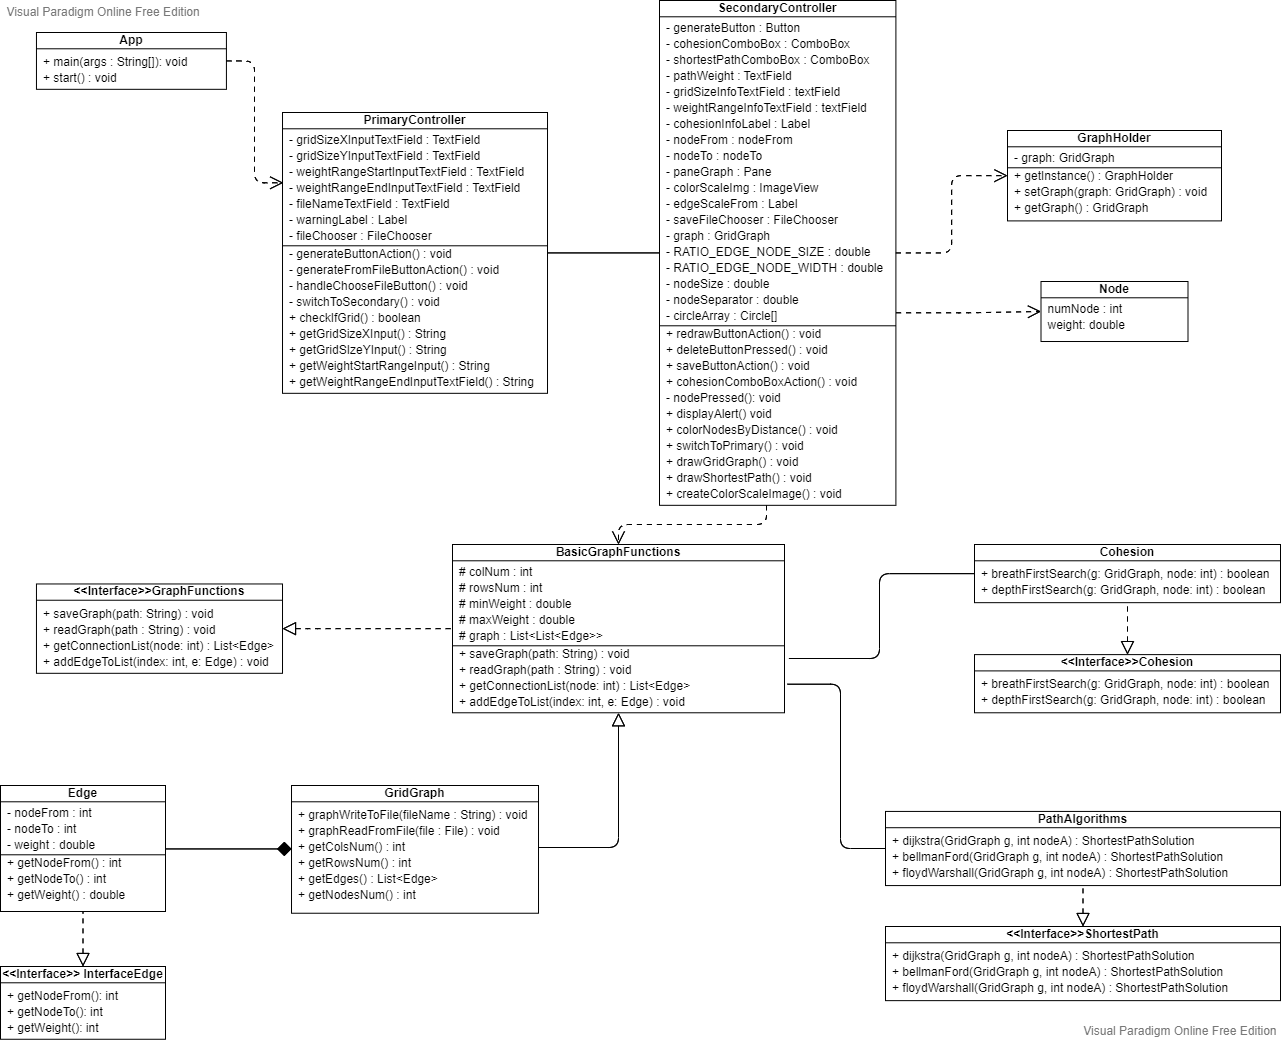
\includegraphics[height=13cm,width=12cm]{Diagram_klas.png}
\caption{Diagram klas projektu \textbf{Grafy}}
\end{figure}
\newpage
\section{Struktury danych}
Zespół do sprawozdania postanowił dodać podaną sekcję i opisać w jaki sposób dane są przechowywane w pamięci komputera:
\begin{itemize}
    \item \textbf{Przechowywanie grafu-}do reprezentacji grafu wykorzystujemy listę sąsiedztwa. Lista sąsiedztwa zamiast zwykłej tablicy jest realizowana za pomocą tablicy list liniowych. Każdy element listy jest strukturą złożoną z numeru wierzchołka, do którego prowadzi krawędź oraz wagi tego połączenia.
    \item \textbf{Breadth First Search-}w celu zaimplementowania algorymtu, zespół użył kolejki FIFO. Kolejka FIFO jest to liniowa struktura danych, w której nowe dane dopisywane są na końcu kolejki, a z początku kolejki pobierane są dane do dalszego przetwarzania.
    \item \textbf{Depth First Search-}przeszukiwanie w głąb polega na badaniu wszystkich krawędzi wychodzących z podanego wierzchołka. Po zbadaniu wszystkich krawędzi wychodzących z danego wierzchołka algorytm powraca do wierzchołka, z którego dany wierzchołek został odwiedzony. W celu zaimplementowania tego algorytmu, zespół wykorzystał stos, dzięki któremu możemy przechowywać numery wierzchołków wychodzących z danego wierzchołka.
    \item \textbf{Dijkstra-}w celu uzyskania lepszej złożoności obliczeniowej algorytmu, zespół wykorzystał kolejkę priorytetową , której implementcja jest w klasie Collections. Kolejka priorytetowa jest kolejką, w której elementy są ułożone nie w kolejności wprowadzania, lecz w kolejności priorytetu. Gwarantuje to pobieranie z kolejki jako pierwszych elementów o najwyższym priorytecie. Elementy o priorytetach niższych zostaną pobrane dopiero wtedy, gdy zostaną usunięte wszystkie elementy o priorytetach wyższych. Kolejka priorytetowa pozwala na szybkie znalezienie najmniejszego połączenia pomiędzy węzłami, co znacznie usprawnia złożoność obliczeniową. Niestety graf, który jest gęsty, czyli np. graf w kratkę, w którym wszystkie węzły są ze sobą połączone nie pokazuje prawdziwej szybkości działania algorytmu Dijkstry z kolejką priorytetową z powodu wysokiej gęstości grafu. Przez wysoką gęstość grafu, algorytm Dijkstry jest bardziej optymalny, używając podejścia naiwnego(bez kolejki priorytetowej) niżeli podejścia z kolejką Priorytetową.
    \newpage
    \item \textbf{Bellman-Ford-}w odróżnieniu do algorytmu Dijkstry, algorytm Bellmana-Forda daje możliwość wyszukiwania najkrótszych ścieżek pomiędzy węzłami w sytuacji, gdy w grafie są ujemne wagi pomiędzy wierzchołkami. Algorytm bellmana-forda jest wolniejszy od algorytmu dijkstry zaimplementowanej w projekcie, ponieważ ma złożoność kwadratową, natomiast dijkstra z kolejką priorytetową złożoność superliniową.
    \item \textbf{Floyd-Warshall-}wykorzystuje metodę programowania dynamicznego. Graf może zawierać gałęzie zarówno o dodatniej i o ujemnej wadze, lecz nie może zawierać ujemnych cykli (cykli, w których suma wag krawędzi jest ujemna). W porównaniu do algorytmów Dijkstry oraz Bellmana-Ford jest to algortym bardzo wolny, ponieważ ma złożoność n*n*n, gdzie n to liczba wierzchołków.
\end{itemize}
\section{Uruchomienie aplikacji}
Zespół postanowił, że wielkość okienka aplikacji będzie ustawiona na 900 x 800 px. Niestety, aplikacja nie ma możliwości automatycznego dostosowywania się do małych ekranów, dlatego na małych ekranach np. laptopach, wygenerowany graf jest bardzo mały. Położenie widoku generacji grafu jest domyślnie ustawione na środek ekranu. Ważnym do dodania aspektem jest mus posiadania przez użytkownika JavaFX, w której stworzone jest GUI. Przenośność aplikacji jest realizowana dzięki Apache Maven 3.8.1. Zespół daje możliwość uruchomienia dwóch metod main w programie:
\begin{itemize}
    \item \textbf{Main w klasie App-} metoda, która umożliwia uruchomienie GUI. W tym trybie użytkownik jest zmuszony, do generowania grafu w kratkę oraz wczytywania grafu, który jest kratką.
    \item \textbf{Main w klasie MainTest-} metoda, która umożliwia uruchoemienie programu w konsoli. Program w konsoli umożliwia dodatkowo wczytanie grafu z pliku, który nie jest kratką. 
\end{itemize}
\newpage
\section{Przykładowe wyniki działania programu}
Przedstawione poniżej wyniki programu prezentują różne podejścia do uruchomienia programu grafy. Prezentujemy możliwości wszystkich zaimplementowanych metod tak, aby bardziej zarysować możliwości programu:
\subsection{Generowanie grafu}
Generowanie grafu w aplikacji odbywa się poprzez podanie wielkości grafu oraz zakresu wag w grafie w kratkę. Po podaniu wszystkich wartości, naciskamy przycisk generate, który spowoduje przejście do sceny obsługującej graf.
\begin{figure}[h]
\centering
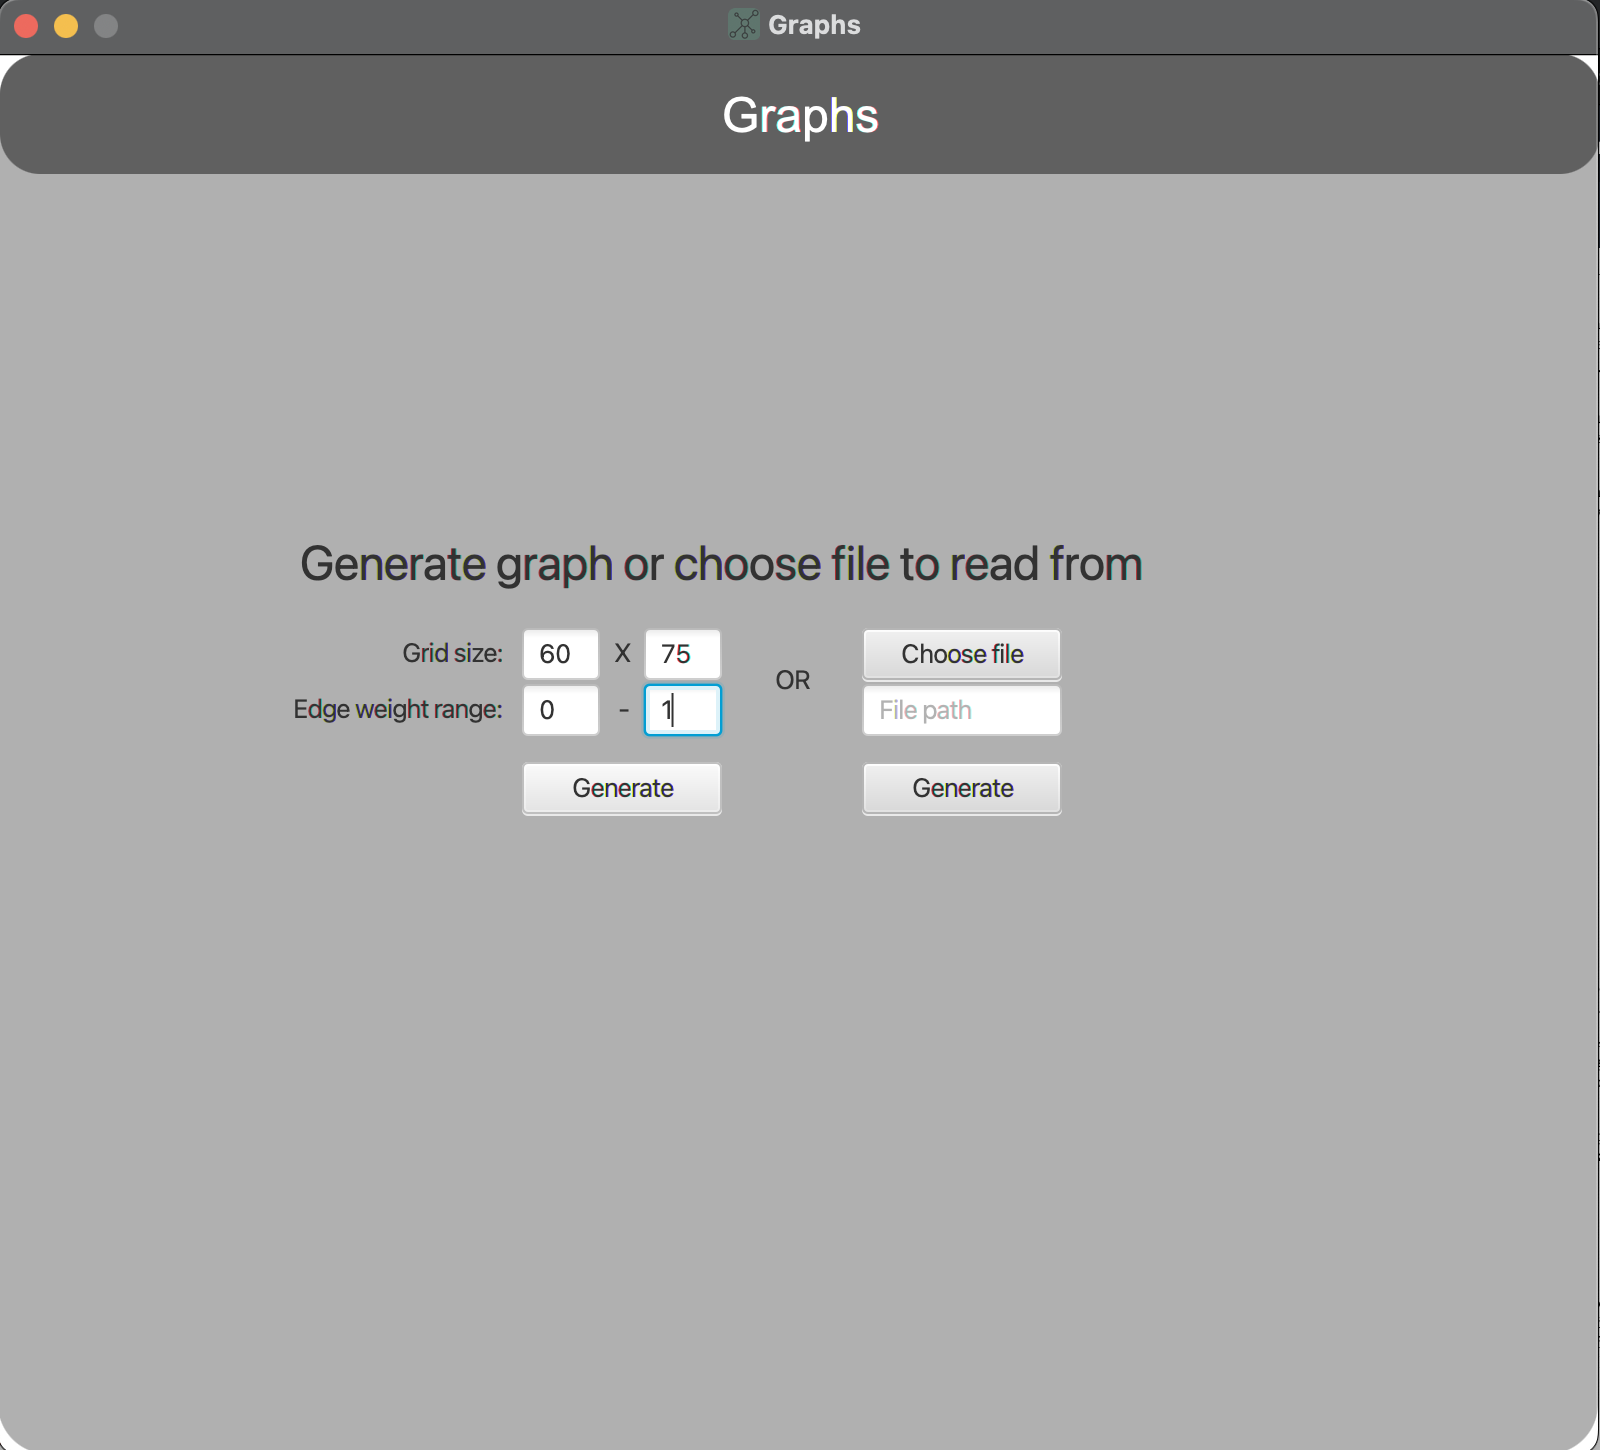
\includegraphics[height=5cm,width=10cm]{Generacja_grafu_widok1.png}
\caption{Widok wpisywania elementów niezbędnych do wygenerowania grafu}
\end{figure}
\begin{figure}[h]
\centering
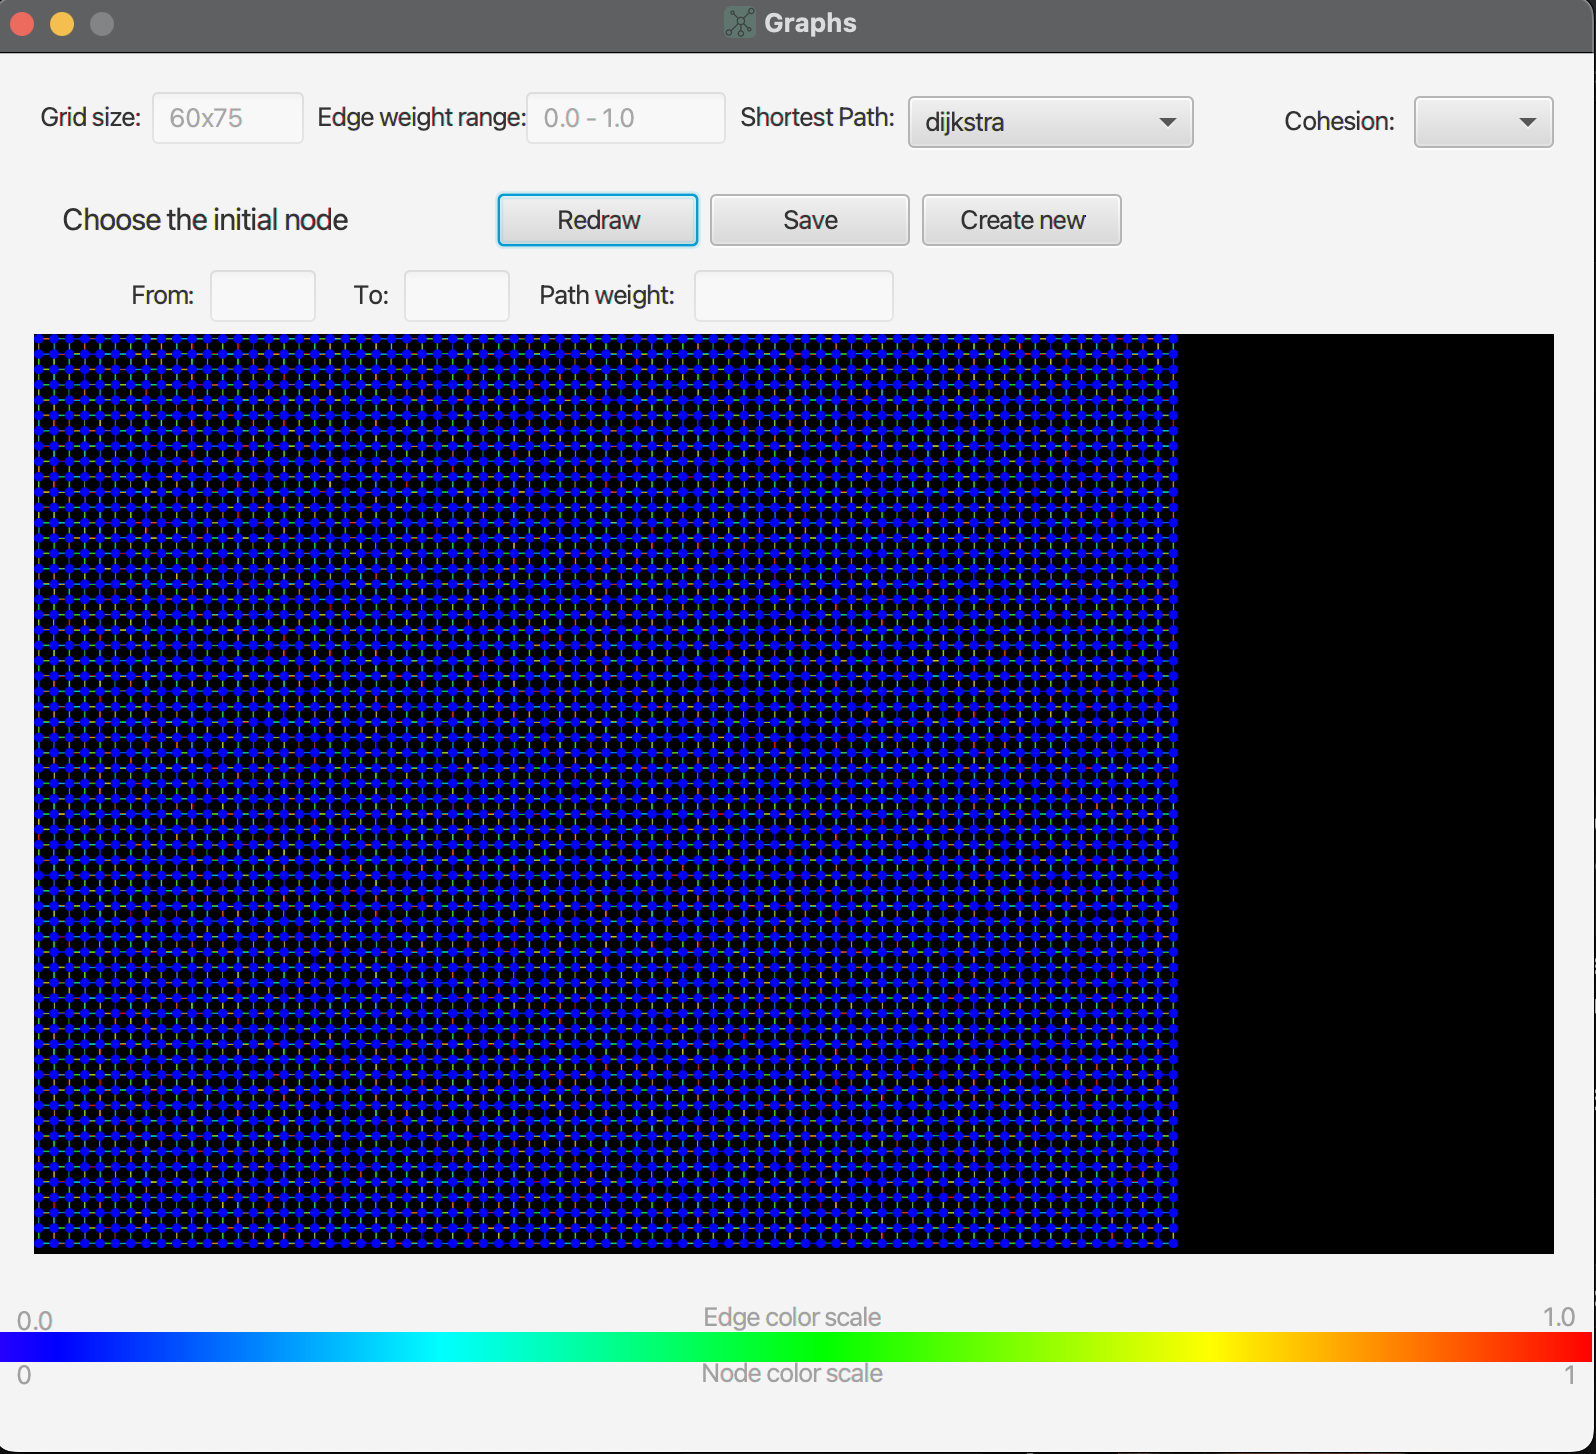
\includegraphics[height=6cm,width=10cm]{Generacja_grafu_widok2.png}
\caption{Widok wygenerowanego grafu na ekranie}
\end{figure}
\newpage
Aplikacja wykrywa również potencjalne złe wartości, które użytkownik może podać przy generowaniu grafu. Przykładem takich wartości może być na przykład niepodanie wag lub liczba kolumn lub wierszy równa 0:
\begin{figure}[h]
\centering
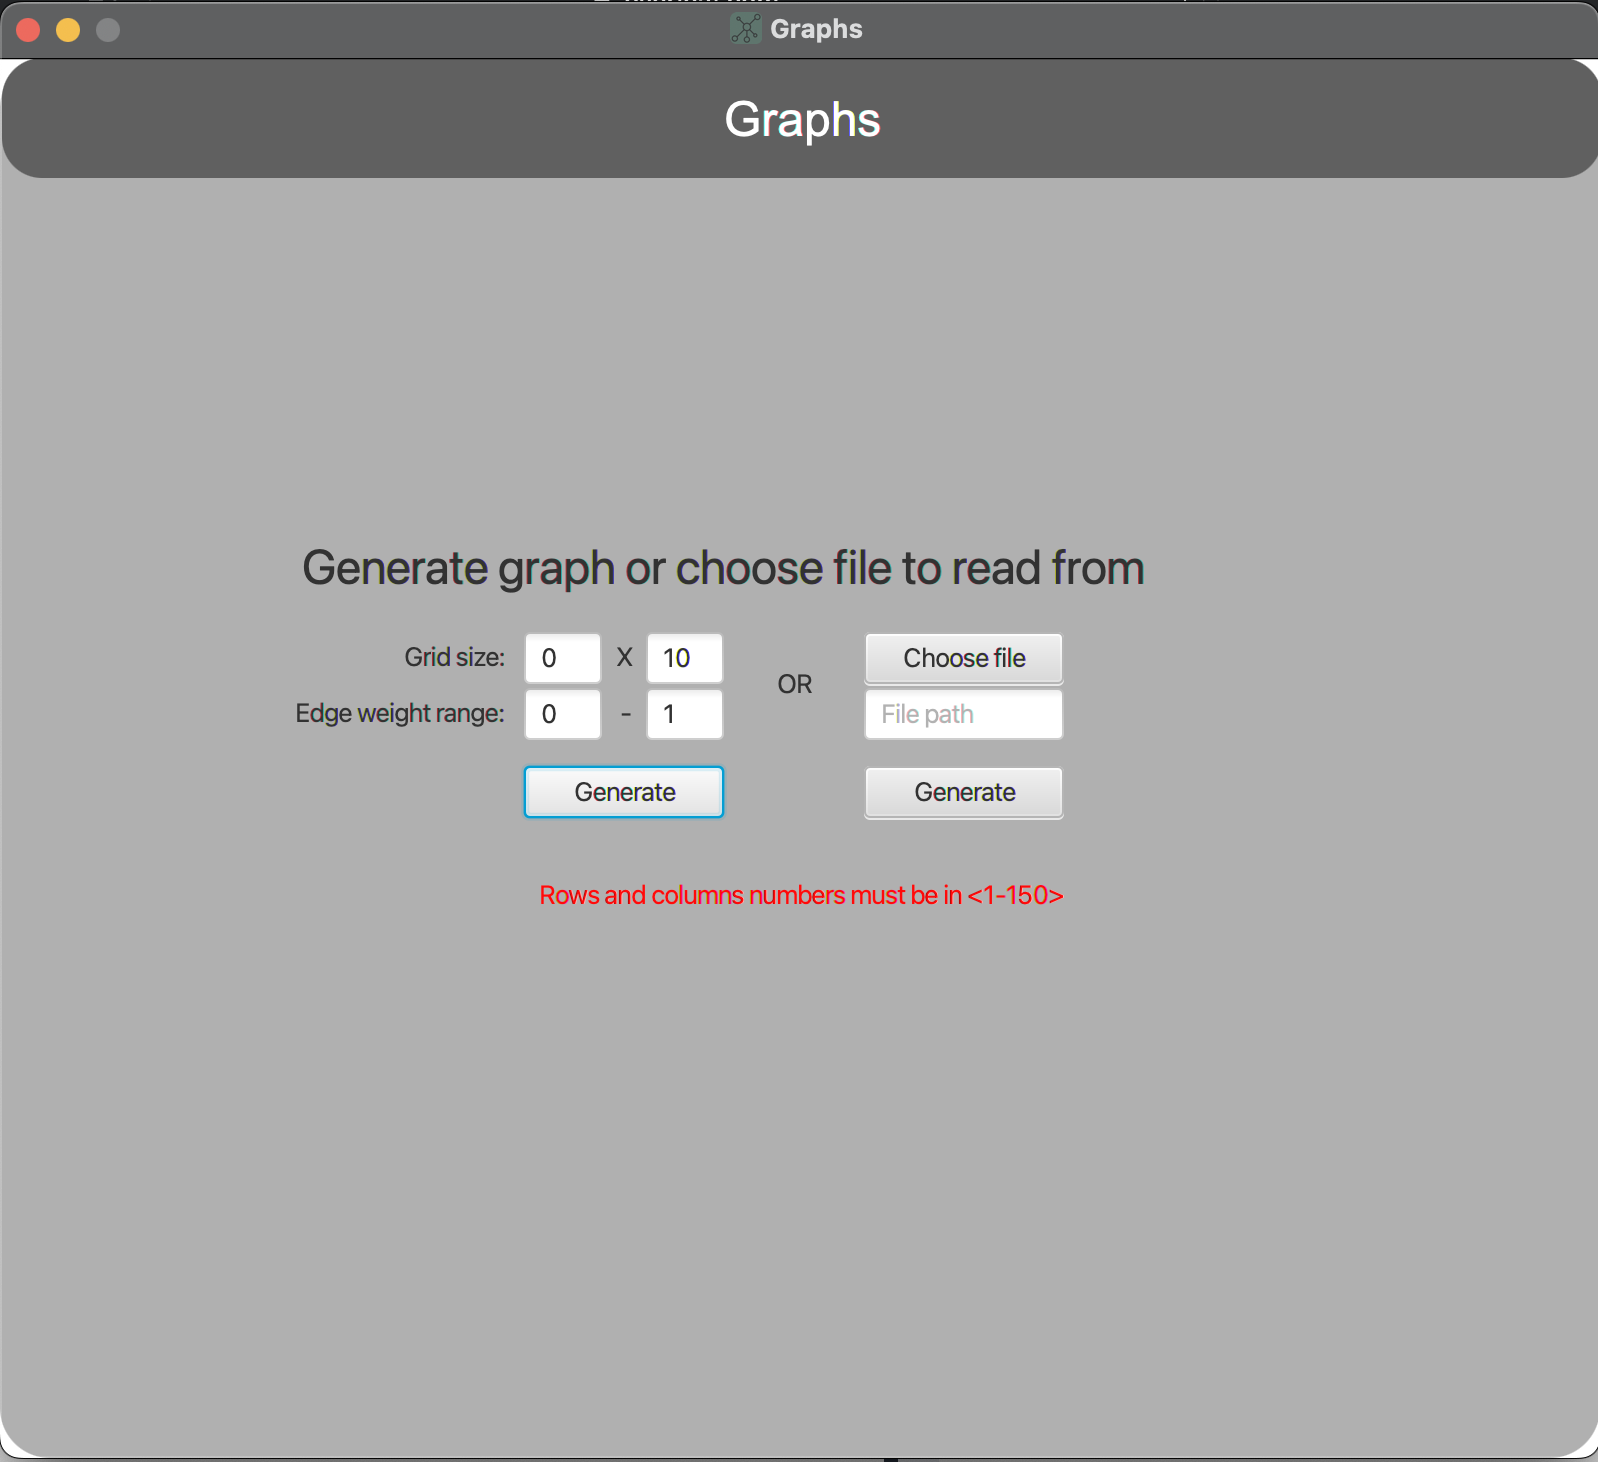
\includegraphics[height=6cm,width=12cm]{Błąd_liczbakolumn.png}
\caption{Błąd - liczba kolumn lub wierszy jest równa 0}
\end{figure}
\begin{figure}[h]
\centering
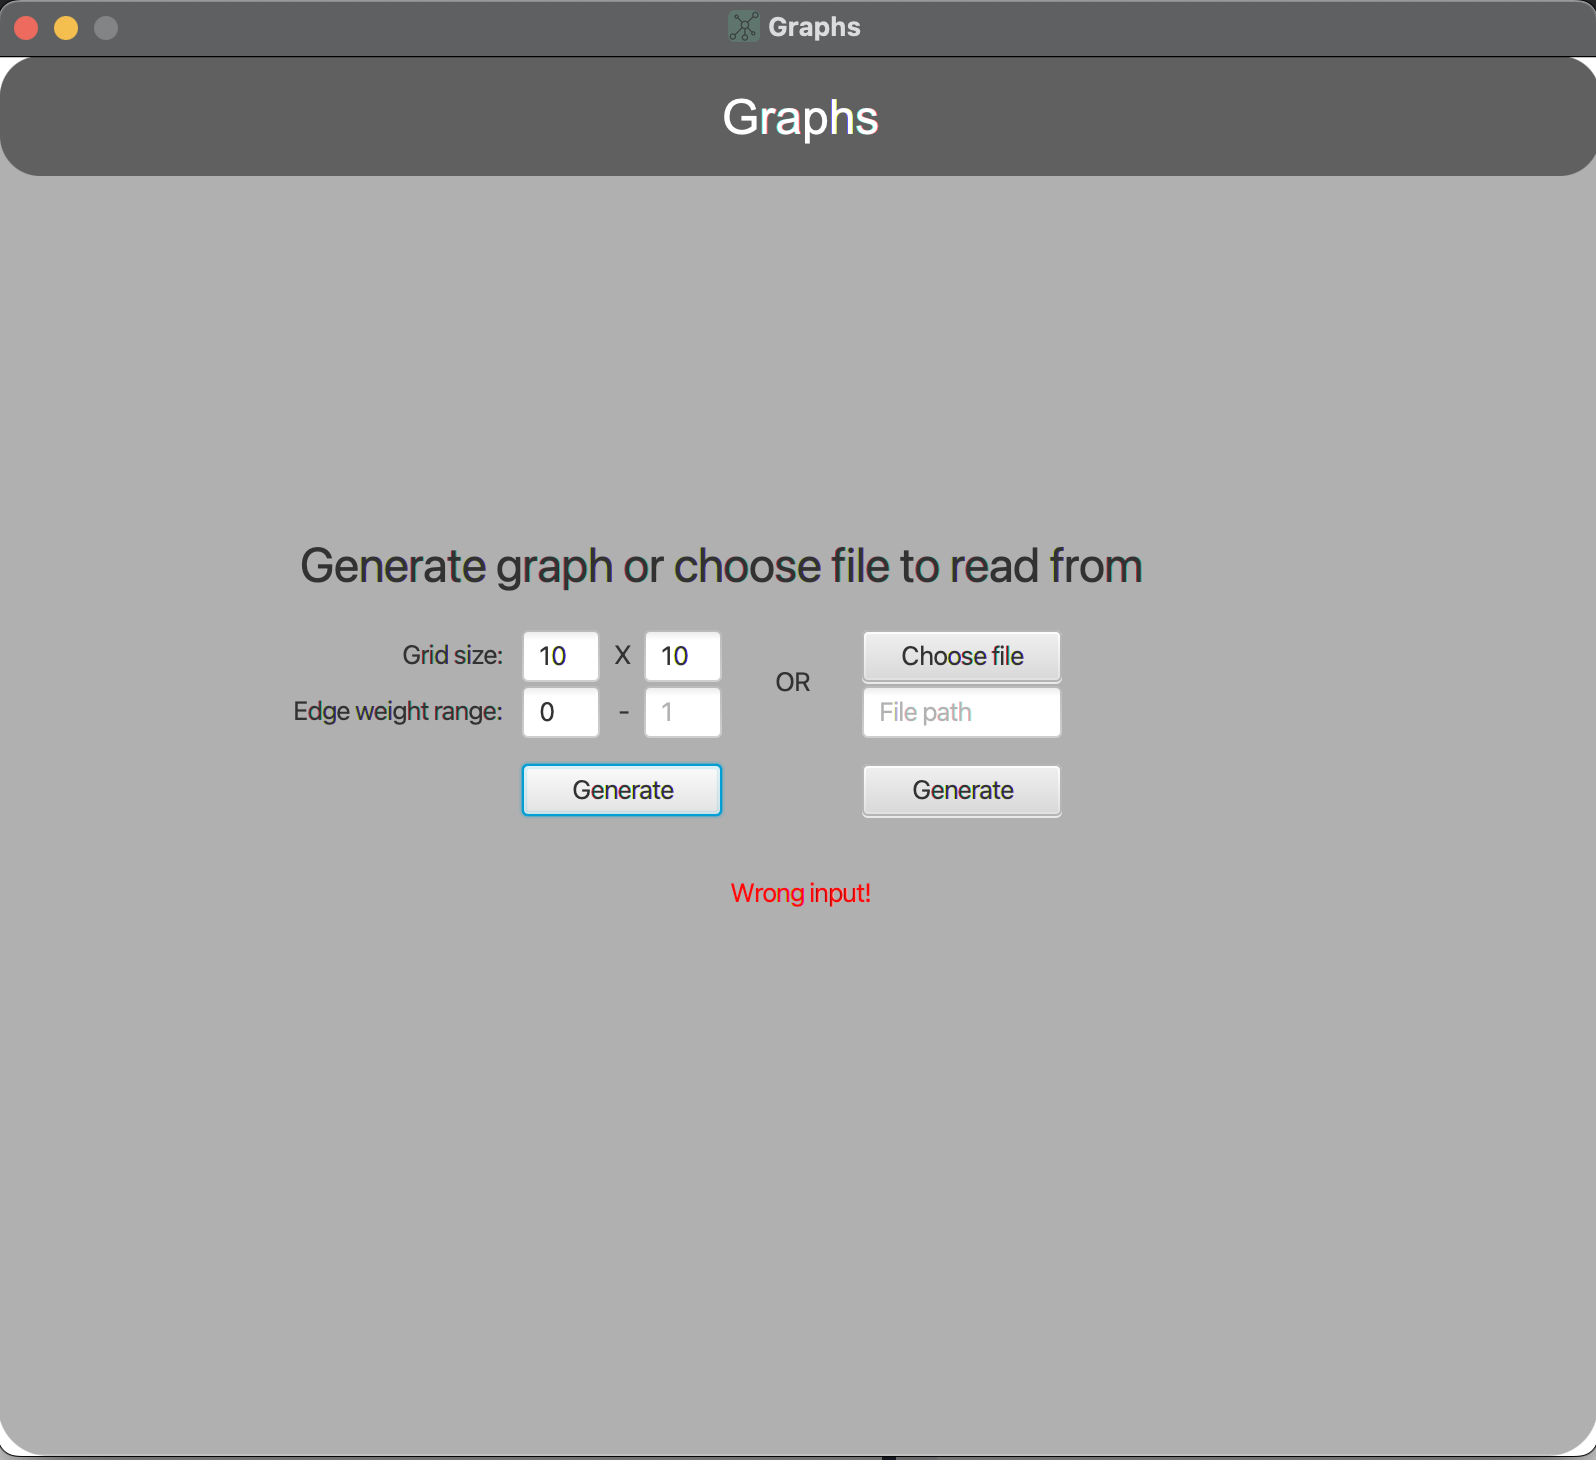
\includegraphics[height=6cm,width=10cm]{Błąd_waga.png}
\caption{Błąd - waga nie została podana}
\end{figure}
\newpage
\subsection{Czytanie z pliku}
Czytanie grafu działa na tej samej zasadzie, co generowanie grafu, tylko na scenie generującej graf, użytkownik musi podać ścieżkę do pliku z przygotowanym grafem w kratkę. Reszta funkcjonalności działa dokładnie tak samo, jak przy generacji. Błędami, jakie mogą wystąpić podczas wczytywania grafu z pliku jest na przykład błąd wczytania grafu, który nie jest w kratkę:
\begin{figure}[h]
\centering
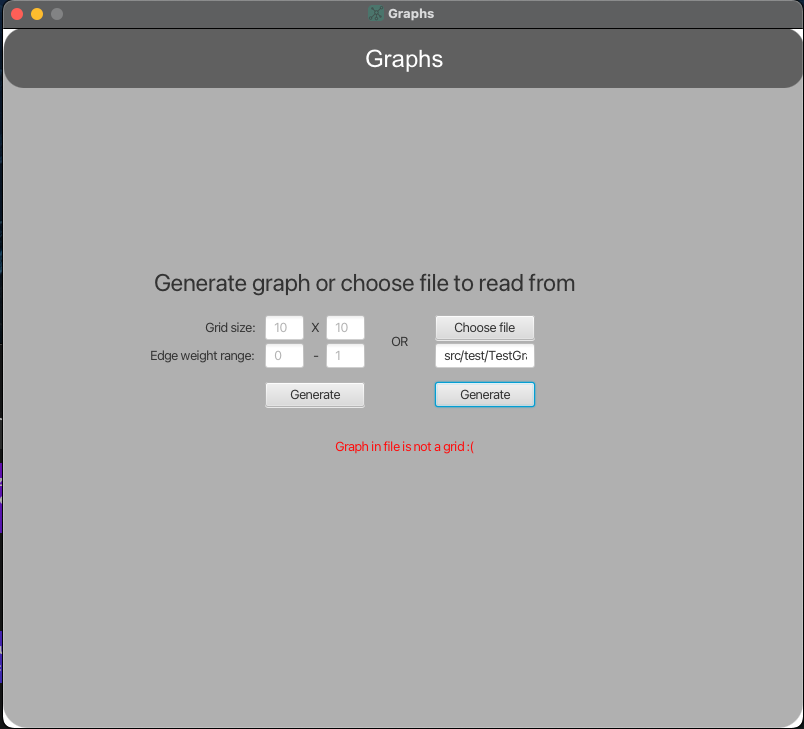
\includegraphics[height=10cm,width=10cm]{Grid_Graph_Error.png}
\caption{Błąd wczytania grafu, który nie jest w kratkę}
\end{figure}
\newpage
\subsection{Algorytmy Bread First Search i Depth First Search}
Algorytm BFS wywołujemy poprzez wybranie z listy algorytmu do badania spójności grafu. Po wybraniu algorytmu, na ekranie wyświetli się informacja o spójności wczytanego grafu. Ważne do dodania jest to, że algorytm wyszukiwania najkrótszej ścieżki w grafie nie będzie działać, jeśli algorytm BFS lub DFS zwrócą informację o niespójności wczytanego grafu:
\begin{figure}[h]
\centering
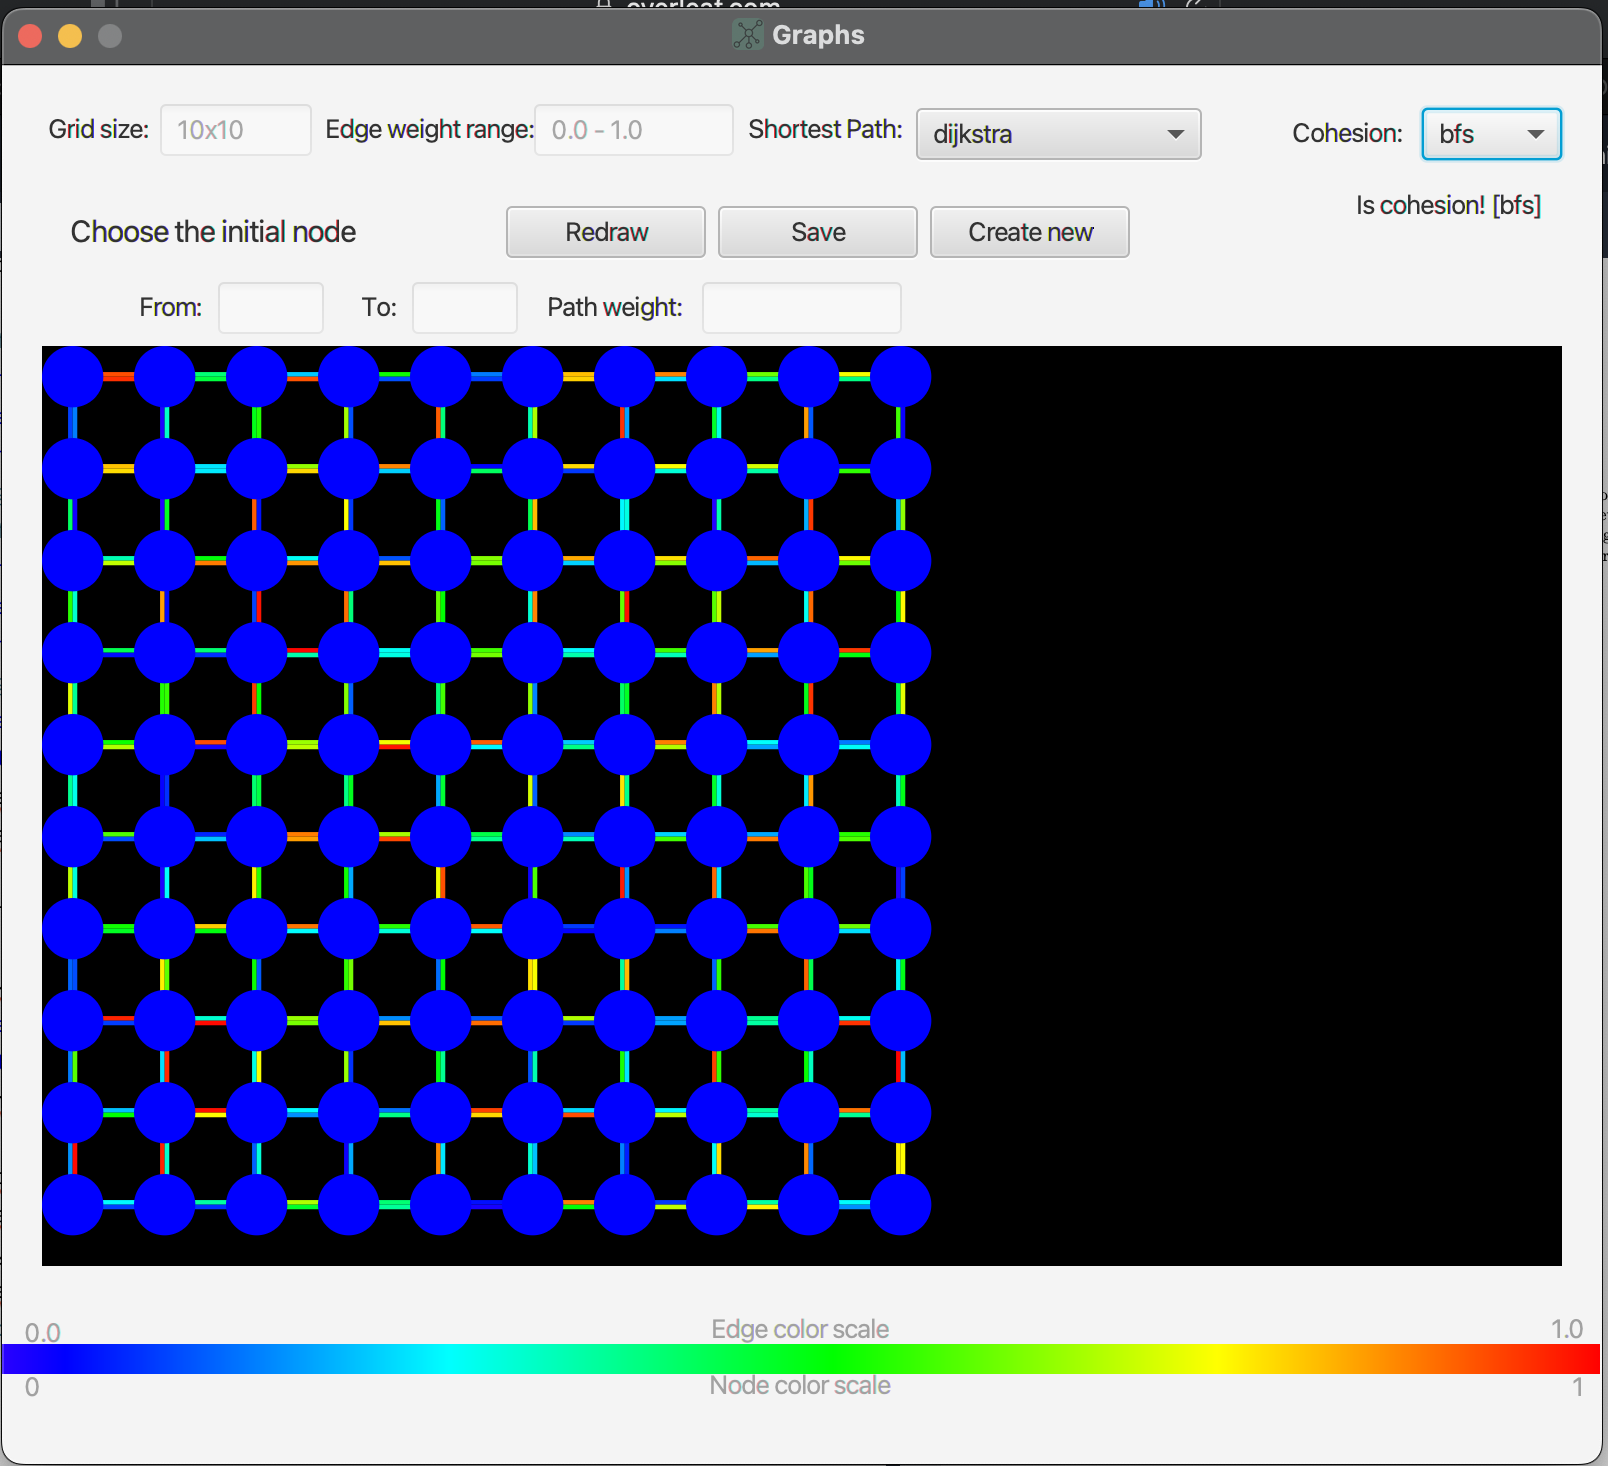
\includegraphics[height=12cm,width=12cm]{BfsDfs_info.png}
\caption{Działanie algorytmu badającego spójność grafu}
\end{figure}
\newpage
\subsection{Algorytmy wyszukujące najkrótszą ścieżkę}
Po wygenerowaniu grafu, aplikacja daje użytkownikowi możliwość uruchomienie działania algorytmów badających spójność lub algorytmów wyszukująych najkrótszą ścieżkę. Podobnie jak w przypadku algorytmu badającego spójność, zespoł postanowił dać użytkownikowi możliwość wyboru jednego z  trzech algorytmów wyszukujących najkrótszą ścieżkę w grafie. Po wybraniu algorytmu(domyślnie jest ustawiona Dijkstra), program prosi o wybranie początkowego wierzchołka. Po wybraniu wierzchołka jesteśmy w stanie wybrać dowolny wierzchołek i zobaczyć na ekranie najkrótszą ścieżkę pomiędzy wybranymi wierzchołkami oraz wagę tego połączenia. Ważną do dodania sprawą jest to, że algorytmy wyszukujące ścieżkę nie zadziałają, jeśli graf jest niespójny.\\ Wygląd grafu po wybraniu wierzchołka początkowego i narysowaniu ścieżki:
\begin{figure}[h]
\centering
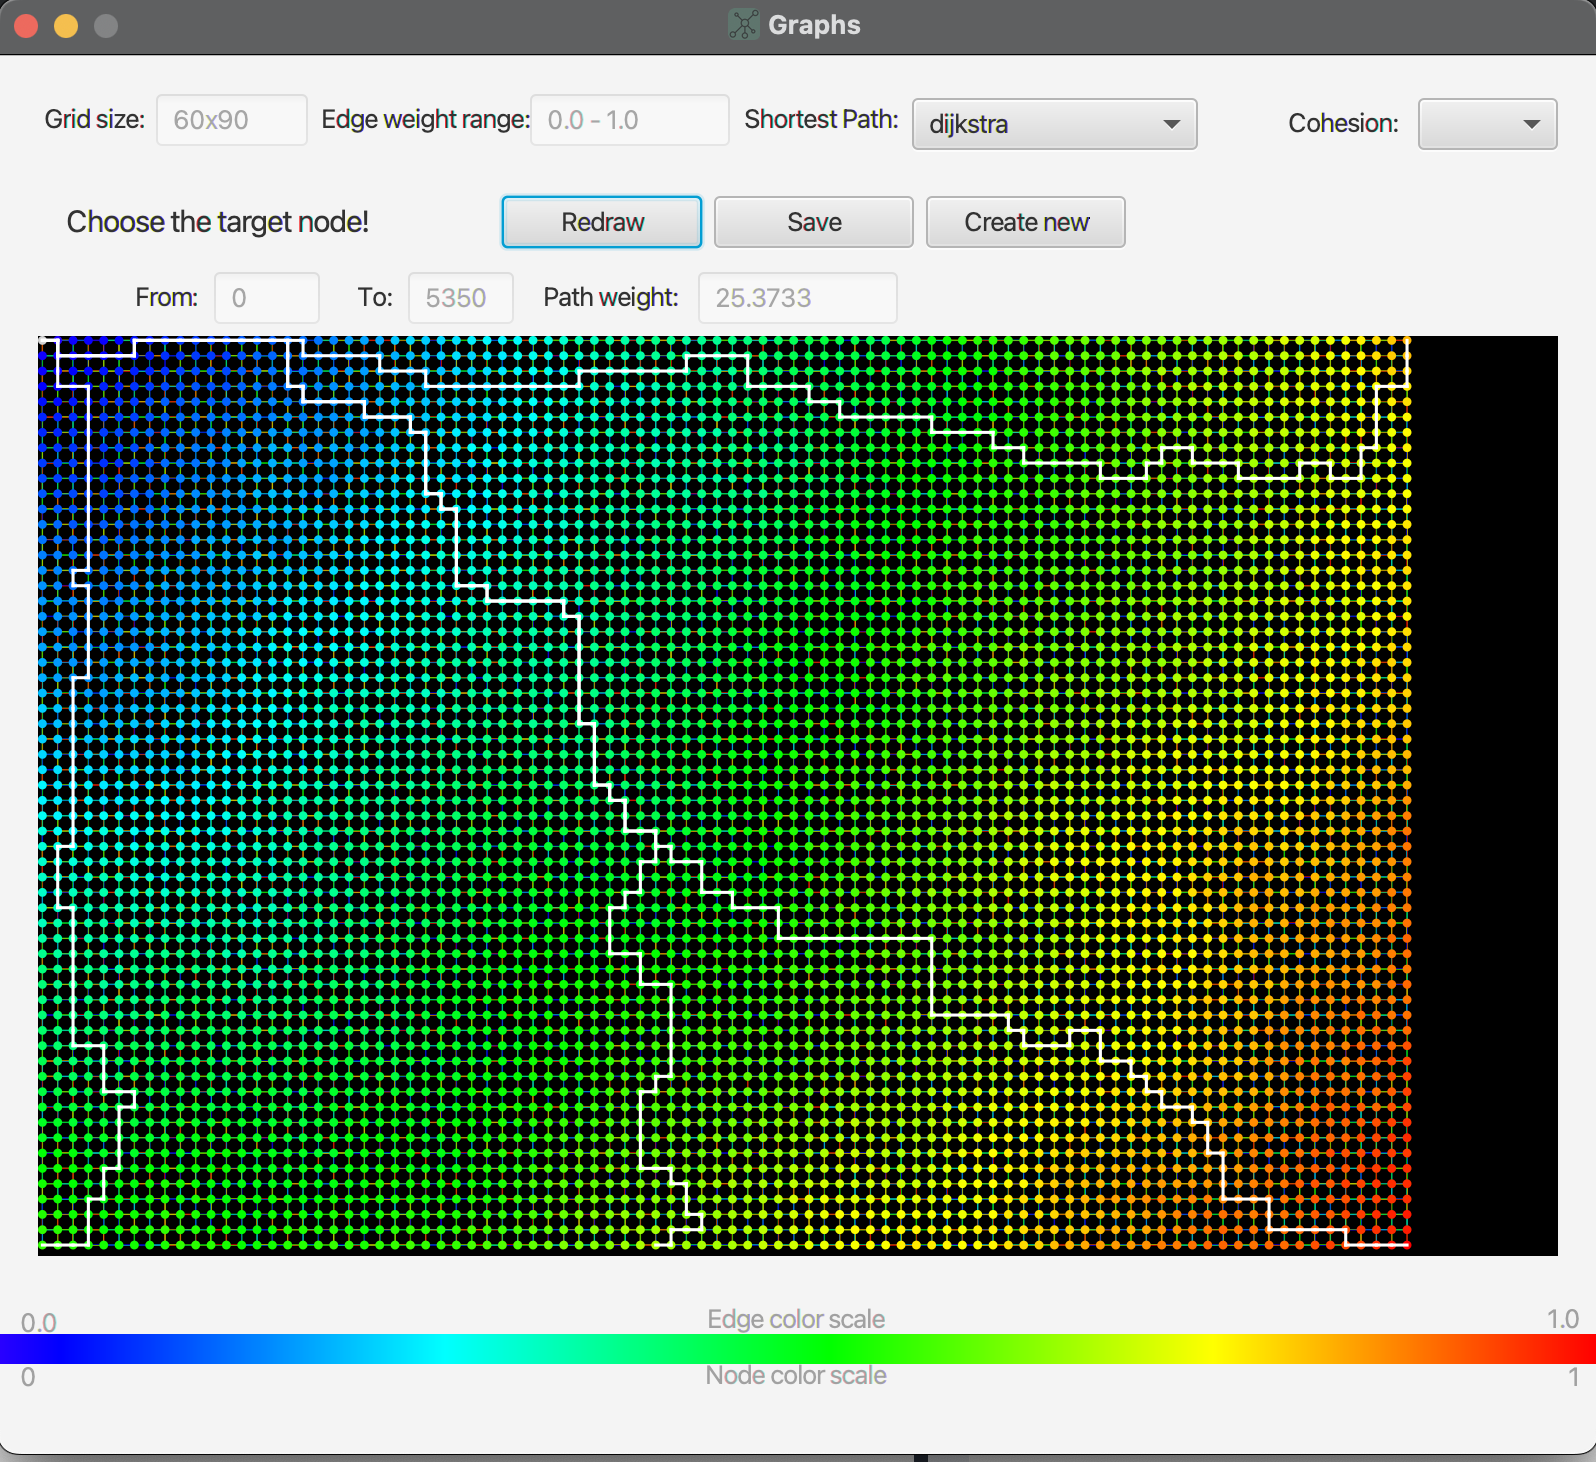
\includegraphics[height=12cm,width=12cm]{Działanie_ścieżka.png}
\caption{Działanie algorytmów wyznaczających najkrótszą ścieżkę}
\end{figure}
\newpage
\section{Zmiany względem specyfikacji implementacyjnej}
Założeniem projektu od momentu zakończenia pisania specyfikacji implementacyjnej było ścisłe trzymanie się planu programu, który był zawarty w specyfikacji implementacyjnej. W procesie powstawania aplikacji praca nad projektem zweryfikowała założone w specyfikacji implementacyjnej idee i skłoniła zespół projektowy do zmiany następujących rzeczy:
\begin{itemize}
    \item \textbf{Zmienienie struktury klas w projekcie-} zmienienie struktury klas w projekcie wynika z małego doświadczenia w programowaniu obiektowym podczas pisania specyfikacji implementacyjnej. Zespół postanowił rozdzielić algorytmy badające spójność i najkrótszą ścieżkę na dwie oddzielne klasy oraz dodać klasę ShortestPathSolution, której instancje przechowują najważniejsze informacje o ścieżkach z poszczególnego wierzchołka w grafie. Dodatkowo zostały dodane interfejsy, zgodnie z praktyką SOLID. Efekt skończonych prac nad strukturą klas w aplikacji został przedstawiony na stronie 3(diagram klas).
    \item \textbf{Zmienienie położenie przycisku generate-} zmiana wynika z wybrania bardziej intuicyjnego dla użytkownika położenia dla przycisku generate.
    \item \textbf{Zmienienie działania przycisku delete-}przycisk delete został całkowicie zastąpiony przyciskiem Create New, który umożliwia usunięcie i wygenerowanie nowego grafu. Ważnym do dodania aspektem jest możliwość zapisania grafu po naciśnięciu przycisku Create New(wyskakuje alert o możliwości zapisu).
\end{itemize}
\newpage
\section{Co było łatwe?}
Podczas całego okresu trwania projektu zespół nie miał problemów z napisaniem możliwości generowania grafu, czytania grafu z pliku tekstowego o ustalonym formacie oraz z algorytmem BFS. Były to stosunkowe łatwe zadania, które nie miały skomplikowanego sposobu działania. Napisanie algorytmów badająych najkrótszą ścieżke pomiędzy wierzchołkami również nie było trudne. Z pomocą przyszły zespołowi rozbudowane biblioteki w Javie, które ułatwiły znaczącą napisanie np. algorytmu Dijkstry z kolejką priorytetową. Stworzenie graficznie GUI również nie było trudne, wszystko realizowało się w Scene Builderze, który jest dość intuicyjnym programem.
\section{Co było trudne?}
Dla zespołu najtrudniejszym zadaniem było napisanie niektórych funkcjonalności w GUI. Najcięższym zadaniem było dostosowanie rozmiaru GUI do ekranu, na którym jest uruchamiany program. Zespołowi ostatecznie udało się to zrealizować, lecz było to ciężkie. Trudne było również przerzucenie się kompletnie z programowania proceduralnego na programowanie obiektowe. Jako zespół omijaliśmy wiele możliwości programowania obiektowego, które wraz z czasem staraliśmy sie dodawać do programu np. Interfejsy.
\section{Co było można zrobić lepiej?}
Zespół jest bardzo zadowolony z funkcjonalności, jakie oferuje program \textbf{Grafy}, lecz zawsze można coś poprawić/zrobić lepiej. Rzeczą, która nie podoba się zespołowi jest brak możliwości dostosowania się generującego się grafu do ekranu. Przy dużych wartościach kolumn i wierszy, graf jest bardzo mały, co powoduje trudności w wyznaczeniu najkrótszej ścieżki. Dostosowanie się aplikacji do wielkości grafu i ekranu są rzeczami, które można by było poprawić.
\section{Podsumowanie pracy nad projektem}
Współpraca zespołowa podczas czasu trwania projektu przebiegała sprawnie i bez większych problemów. Problemem, który w pewnym momencie projektu zatrzymał zespół w działaniu był brak umiejętności programowania w JavieFX. Po obejrzeniu poradników oraz pracy z dokumentacją, zespół był w stanie zacząć pisać GUI. Wartym odnotowania współczynnikiem, który wpłynął na wydajność pracy zespołu było korzystanie z systemu kontroli wersji git. Dzięki systemowi kontroli wersji, zespół mógł sprawnie wymieniać się aktualnymi wersjami programu oraz analizować dokonane przez współpracownika zmiany w programie. Pomocne były także konsultacje projektowe, na których członkowie zespołu wyjaśniali zastosowane w programie rozwiązania oraz przydzielali sobie kolejne zadania. Pomagało to znacznie zorganizować pracę i zrozumieć program pod kątem konceptualnym. Podsumowując, współpraca projektowa była na zadowalającym poziomie mimo drobnych błędów i pozwalała na wspólne rozwiązanie problemu i uczenie się efektywnej pracy w zespole programistycznym.
\section{Podsumowanie projektu}
Projekt \textbf{Grafy} został całkowicie zrealizowany w dniach 01.04.2022 do 02.06.2022 przez Adriana Nowosielskiego oraz Cezarego Skorupskiego. W trakcie tego okresu zespołowi udało się stworzyć dokumentację składającą się ze specyfikacji implementacyjnej oraz sprawozdania końcowego oraz działający program GRAFY w języku Java z działającym graficznym interfejsem użytkownika. W celu zwiększenia intuicyjności poruszania się po programie, zespół opisuje każdy przycisk oraz dobiera poprawną kolorystykę. Dodatkowo, w celu sprawdzenia funkcjonalności, zespół dostarcza 15 niezależnych od siebie testów jednostkowych rozwiązań zastosowanych w projekcie. Testy jednostkowe zostały wykonane w technologii JUnit. W konsekwencji pracy nad testowaniem aplikacji, działanie programu powinno być maksymalnie zgodne z oczekiwaniami.
\section{Podział pracy w zespole}
W tej sekcji przedstawimy tylko najważniejsze podziały pracy w zespole. Podczas projektu, staraliśmy się pracować razem nad problemami, dlatego w niektórych zadaniach jest wpisane, że zadanie zostało wykonane wspólnie, ponieważ nie robiła tego tylko jedna osoba. Podczas trwania projektu, zespół starał się pracować razem, by pracować efektywnej nad kodem i wiedzieć co się dzieje w danym momencie trwania projektu:\\
\textbf{Specyfikacja implementacyjna-} Zadanie wspólne\\
\textbf{Generowanie grafu-} Adrian Nowosielski\\
\textbf{Czytanie grafu z pliku-} Adrian Nowosielski\\
\textbf{Algorytmy badające spójność-} Adrian Nowosielski\\
\textbf{Algorytmy wyznaczające najkrótszą ścieżkę-} Adrian Nowosielski\\
\textbf{Testowanie programu-} Adrian Nowosielski\\
\textbf{Wprowadzenie kontroli błędów do programu-} Adrian Nowosielski\\
\textbf{Stworzenie widoków w Scene Builderze-} Cezary Skorupski\\
\textbf{Generacja grafu w GUI-} Cezary Skorupski\\
\textbf{Wyznaczanie najkrótszej ścieżki na ekranie-} Cezary Skorupski\\
\textbf{Wprowadzenie kontroli błędów w GUI-} Cezary Skorupski\\
\textbf{Wprowadzenie gradientu wagi scieżek-} Cezary Skorupski\\
\textbf{Sprawozdanie-} Zadanie wspólne
\newpage
\section{Wnioski}
Projekt \textbf{Grafy} jest zadaniem, które pozwala na różnorodne podejście do problemu grafu i zaimplementowanie różnych rozwiązań, które znacznie wpłyną na szybkość oraz działanie programu. W przypadku algorytmu Dijkstra, czyli algorytmu, który może przeszukiwać grafy o bardzo dużej liczbie wierzchołków, pomocne jest zastosowanie narzędzia, które maksymalnie zmniejszy czas wyszukiwania najkrótszego połączania pomiędzy wybranymi wierzchołkami. Użyte w programie podejście do algorytmu Dijkstry poprzez kolejkę priorytetową pozwoliło ograniczyć problem szybkości działania algorytmu. Istotnym aspektem godnym poruszenia jest duża liczba testów wykonanych przez zespół, co pozwoliło w łatwy sposób znajdować błędy i je eliminować. Projekt pozwolił zespołowi poznać techniki programowania obiektowego i wykorzystać je w praktyce. Zespół podczas pisania rozwiązania projektu, starał się korzystać z dobrych praktyk programistycznych SOLID. W tworzeniu graficznego interfejsu użytkownika, zespołowi pomógł program SceneBuilder, w którym niemal automatycznie tworzy się wygląd sceny, do której wystarczy napisać funkcjonalności takie jak np. rysowanie ścieżki. W ogólnym rozrachunku, zespół jest zadowolony z dostarczonego projektu oraz z umiejętności nabytych podczas programowania rozwiązania programu \textbf{Grafy}. 
\end{document}